\documentclass[]{article}

%opening
\title{Simulated Instrumental Constraints on Sub-Stellar Atmospheric Retrievals for the JWST's Mid Infrared Instrument.}
\author{Evert Nasedkin}

\usepackage[style=ieee,hyperref]{biblatex}

\usepackage{graphicx}
\usepackage{microtype}
\usepackage{bm}
\usepackage{listings}
\usepackage{url}
\usepackage{tikz}
\usetikzlibrary{shapes,arrows}
\usepackage{booktabs}
\usepackage{pdfpages} 
\usepackage[top = 1in, bottom = 1in, left = 1in, right = 1in]{geometry}
\bibliography{thesis_bib}
\begin{document}
\graphicspath{{figures/}}
\maketitle
\begin{abstract}
Following its launch in 2021, the James Webb Telescope will provide the best infrared observations of exoplanets and brown dwarfs to date.
In particular, the Mid-Infrared Instrument (MIRI) will allow for medium resolution spectroscopy from 4.9-28.8$\mu$m.
This thesis improves the implementation of a thin-film fringing model for point sources to MIRISIM, considering how the fringing effect from the detector layers varies with the focal plane position of a point source. 
Understanding such instrumental effects is key to quantifying the ability of MIRI to derive atmospheric properties, which will be characterized by an atmospheric retrieval study.
Existing literature has considered the NIRCAM instrument and the MIRI Low-Resolution Spectrometer, but it is critical to extend wavelength coverage to the mid-infrared to improve the results of an atmospheric retrieval. 
The longer wavelength range allows measurement of abundances of species inaccessible at shorter wavelengths, such as NH$_{3}$, and improvements to measurements of H$_{2}$O, CH$_{4}$, CO$_{2}$ and others.
\end{abstract}
\vspace{0em}
\begin{figure}[h]
	\centering	
	\begin{minipage}{0.45\linewidth}
	\centering
	\vspace{-1em}
	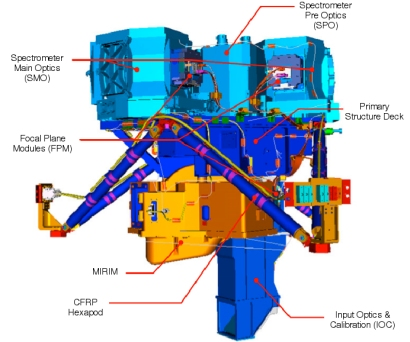
\includegraphics[width=\linewidth]{MIRI.jpg}		
	\caption{The MIRI Medium Resolution Spectrograph \cite{Wells2015} is an Integrated Field Spectrograph on the James Webb Space Telescope with R$\approx$3000 and wavelength coverage from 4.8-28.8$\mu$m. This will allow for the characterization of brown dwarf and exoplanet atmospheres in a previously inaccessible regime. While the performance of MIRI is unprecedented, it is still limited by instrumental effects. Image courtesy ESA and the University of Leicester.}
	\end{minipage}
	\hspace{2em}
	\begin{minipage}{0.45\linewidth}
	\centering
	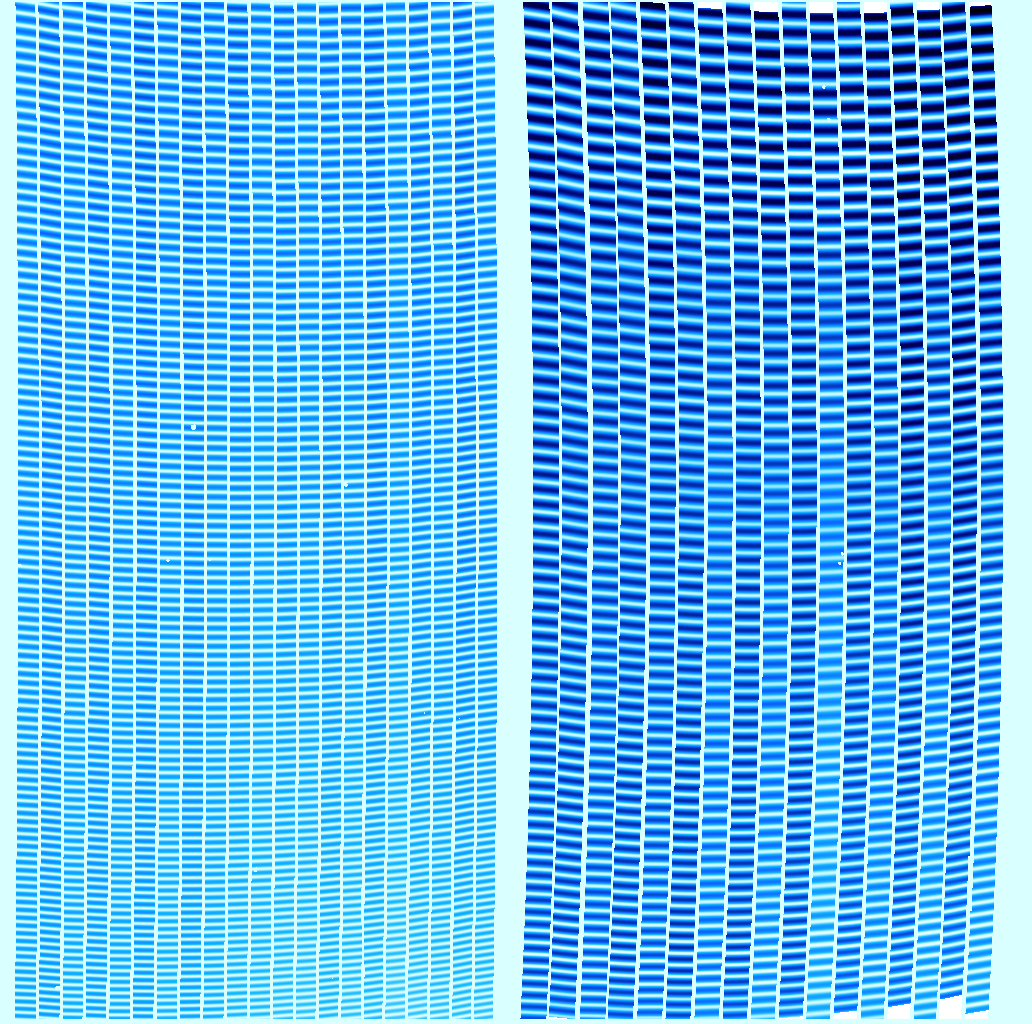
\includegraphics[width=0.95\linewidth]{CVFringeFlat.png}	
	\caption{Of particular interest to atmospheric characterization is the wavelength dependent fringing effect, caused by thin-film interference from the multiple layers used to construct the detectors \cite{Argyriou2018a}. This effect is not yet fully understood, nor fully implemented in the instrumental simulator. The primary goal of this project is to understand the impact of this effect on atmospheric retrievals. Shown: A fringe flat that is applied to the light projected onto the MRS detectors in the instrumental simulator .}	
	\end{minipage}
\end{figure}
\begin{figure}[h]
	\centering
	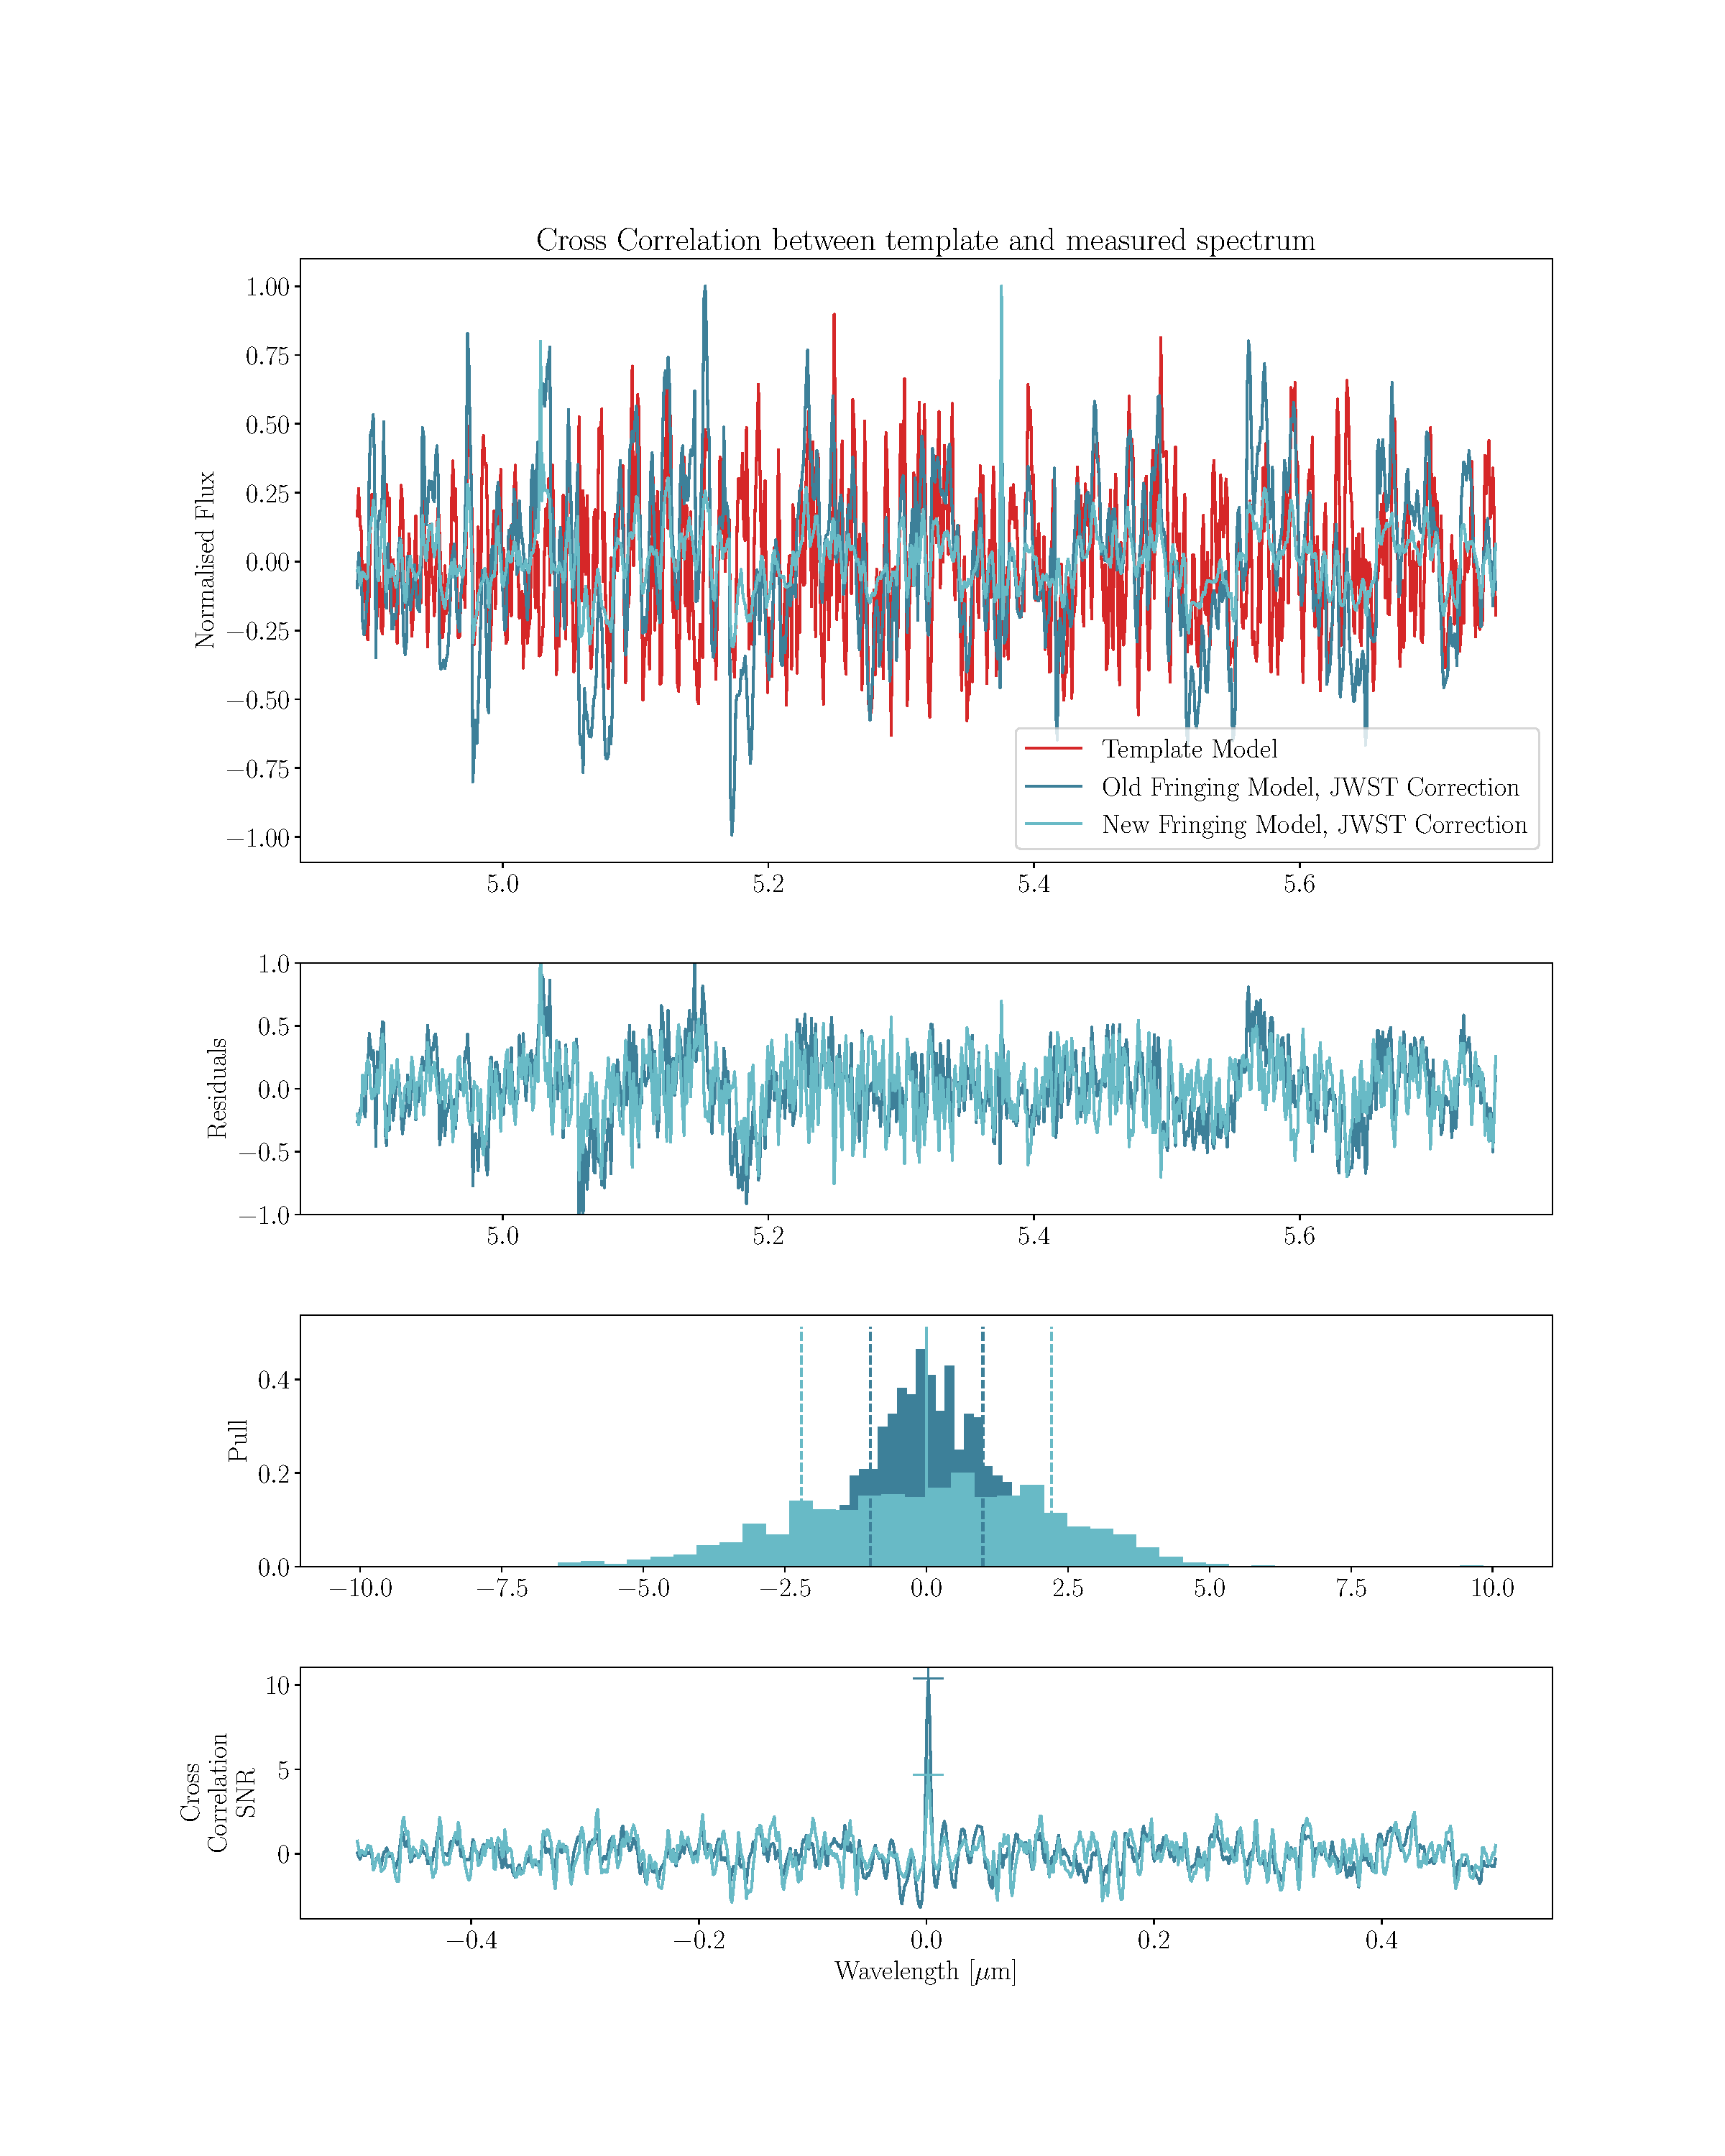
\includegraphics[width=\linewidth, trim = 2cm 3cm 1cm 5cm,scale = 1.2]{hr8799e15pc_offaxnewold_cor_v1}
	\caption{To quantify the fringing effect we use the cross-correlation method to measure the similarity of an extracted spectrum to an input template. \textbf{1.} Artificial atmospheric spectra from \cite{Molliere2019} are processed using the MIRISIM instrumental simulator \cite{Consortium2018}, and retrieved using the standard JWST pipeline \cite{Bushouse2015}. We compare the use of a fringe flat derived from focal plane position dependent point-source FM data to the standard MIRISIM fringe flat from the CV campaign which used an extended source. \textbf{2.} The residuals of the normalized input template subtracted from the extracted spectra. \textbf{3.} We find that the distribution of the residuals of the point-source derived flat is wider. \textbf{4.} We find that the more representative point-source data results in a decrease in the signal-to-noise ratio of the cross correlation, demonstrating that this effect will impact measurements of spectra unless properly corrected using an optical model or improved calibration data \cite{Argyriou2018}.}
\end{figure}
\begin{figure}[h]
	\centering
	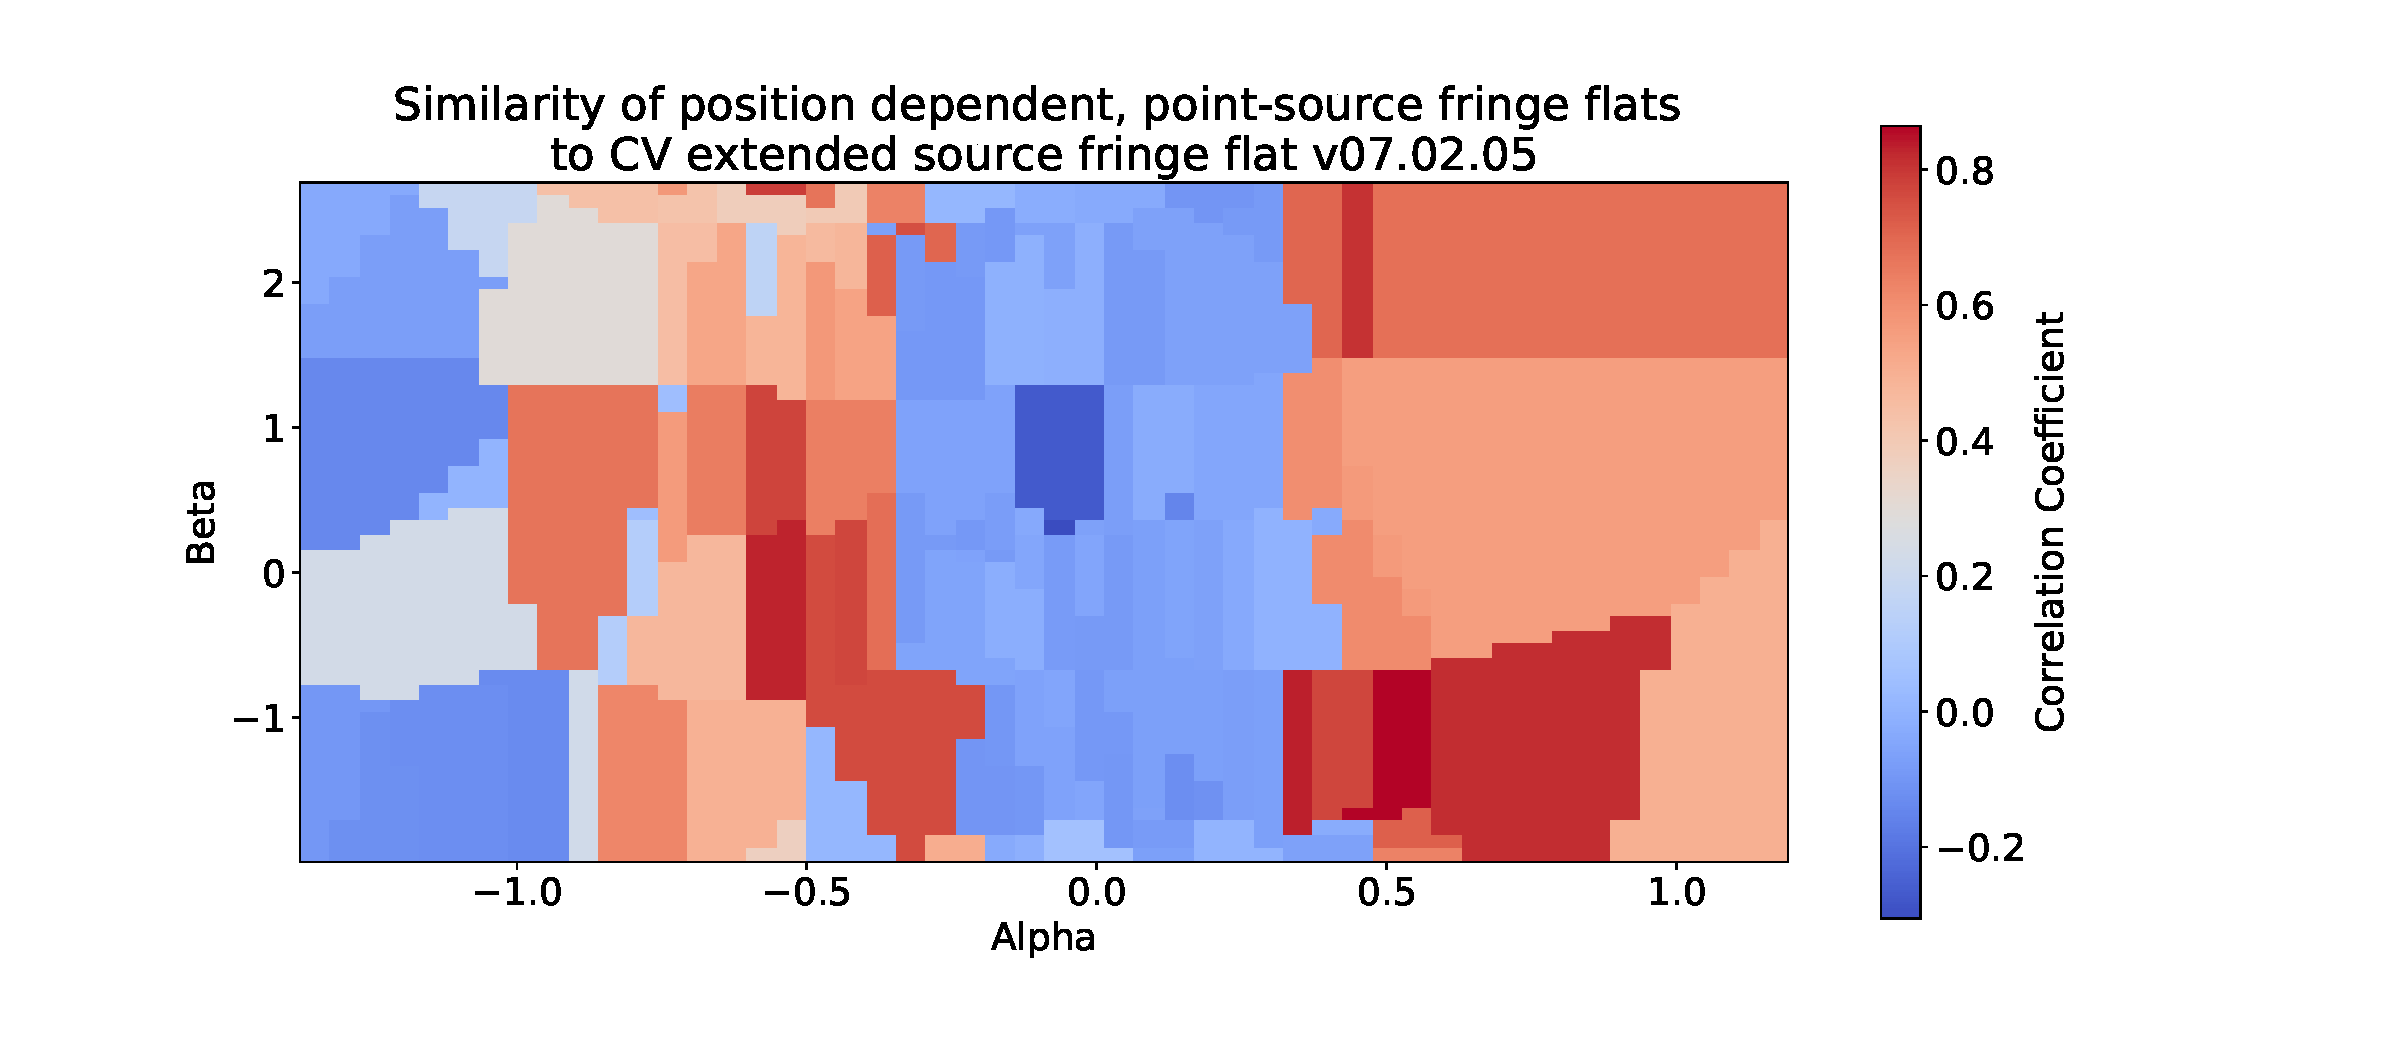
\includegraphics[width=\linewidth,trim = 2cm 0.5cm 4cm 5cm]{PosnCor_v5}
	\caption{We examine the variation of the fringing signal as a function of the position of the point source in the focal $(\alpha,\beta)$ plane. We measure the correlation between the point source fringe spectrum and the standard extended source fringe spectrum at the same location. While there is a clear radial trend in the similarity of the spectra, the nature of this relationship has not yet been determined.}
\end{figure}
\begin{figure}[h]
	\centering
	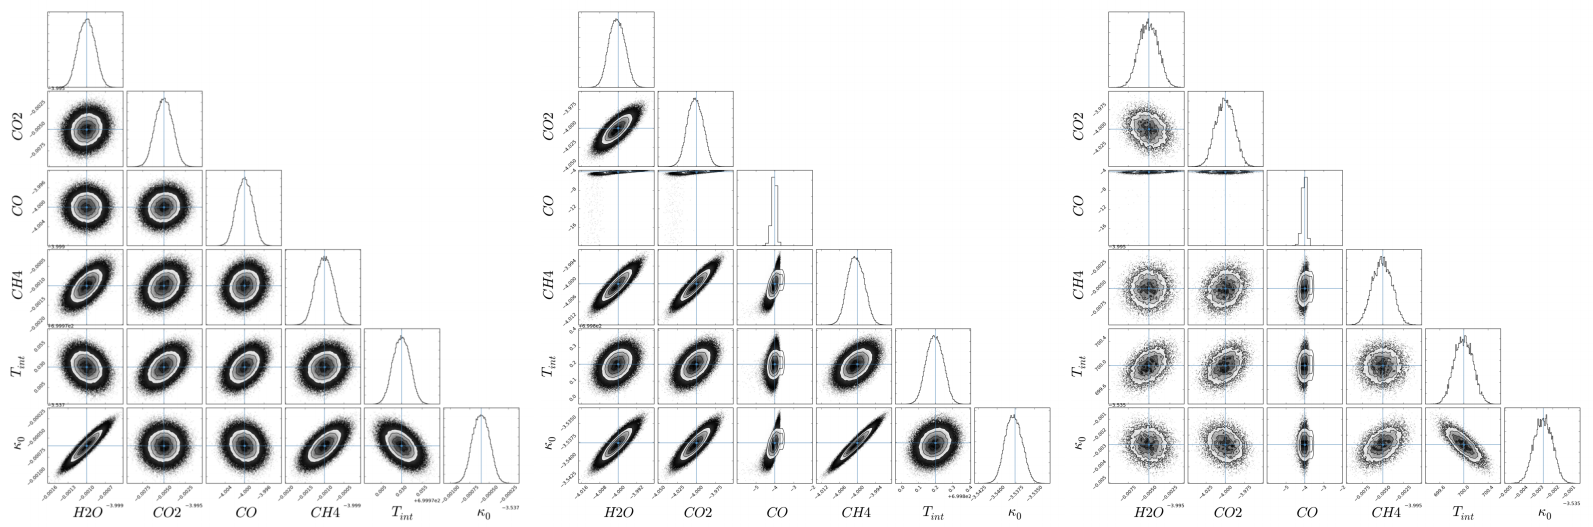
\includegraphics[width=\linewidth]{HeliosExample.png}
	\caption{Going forward, we will measure the impact of this effect on the science goals of an atmospheric retrieval, determining the impact on the widths of the posterior distributions for temperature, log g and composition. In general, this will also allow us to examine the ability of MIRI to retrieve this parameters either alone or when combined with shorter wavelength data \cite{Schlawin2018, Batalha2018}. This will be accomplished using the petitRadTrans code \cite{Molliere2019} to generate the spectrum, and using a nested-sampling approach based on the HELIOS retrieval code \cite{Lavie2017}. Shown: Example of posterior distributions for chemical species generated by a HELIOS atmospheric retrieval \cite{Lavie2017}.}
\end{figure}
\clearpage
\printbibliography
\end{document}
